{\bf Introduction}

In this assignment we will be working on a sentiment classification for the movies. We will build a binary linear classifier that reads movie reviews, as you would see from the sites like Rotten Tomatoes, and predicts whether the result is positive or negative.

Rotten Tomatoes has classified these reviews as "positive" and "negative", respectively, as indicated by the intact tomato on the left and the splattered tomato on the right. In this assignment, you will create a simple text classification system that can perform this task automatically.

Here are two reviews of Minari \url{https://www.rottentomatoes.com/m/minari/reviews}, courtesy of Rotten Tomatoes (no spoilers!):


\begin{figure}[h]
    \begin{center}
        \captionsetup{width=0.8\textwidth}
        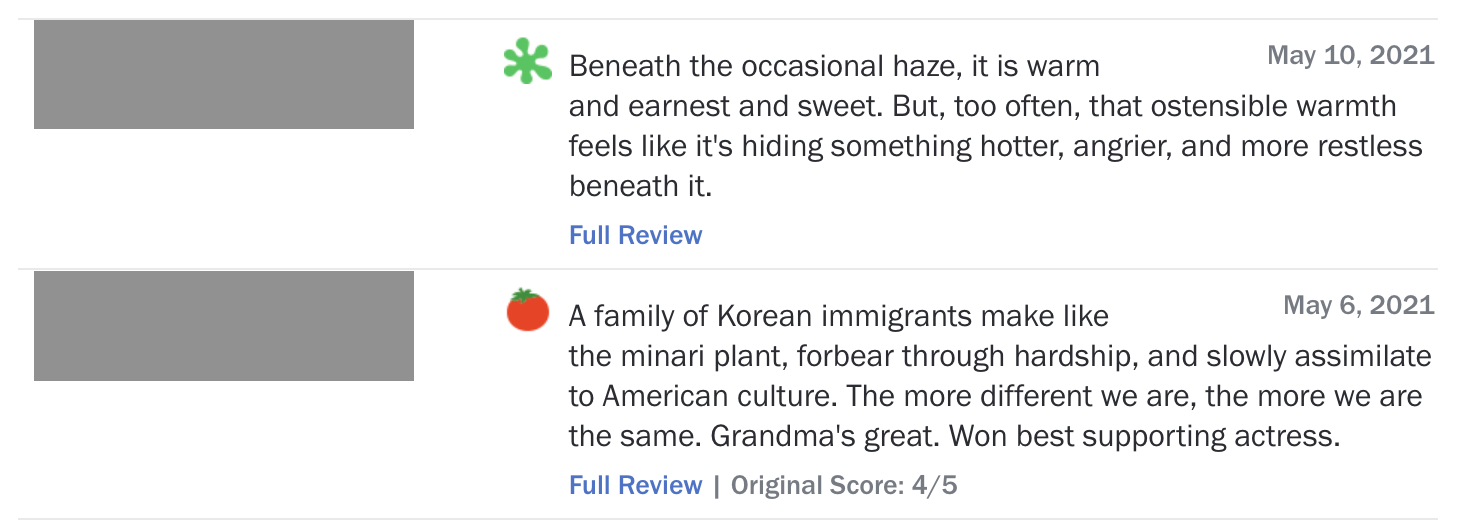
\includegraphics[width=0.7\textwidth]{images/minari.png}
        \caption{Here are positive and negative reviews of Minari, from Rotten Tomatoes}
        \label{rotton_tomatoespos}
    \end{center}
\end{figure}


Advice for this assignment:
\begin{itemize}
  \item In the context of this assignment, words are simply strings separated
  by whitespace. This includes case and punctuation (e.g. ``great'' and
  ``Great'' are considered different words).
  \item You might find some useful functions in |util.py|.  Have a look
  around in there before you start coding.
\end{itemize}
